% !TEX root = ../main.tex
%
\chapter{Health State Classification}
\label{sec:system}

\cleanchapterquote{A healthy outside starts from the inside.}{Robert Urich}{(Actor)}\newline 
\vspace*{-15mm}
\hfill{\fontfamily{phv}\normalsize\emph{Anurose Prakash}}\newline 
\newline 

In the entire life cycle of industrial machinery, the machines undergo a series of health degradation states from time to time till it reaches to a complete failure state. The historical knowledge of the health transition associated with the existing machinery can be used to predict the upcoming changes that the same machinery will undergo. This is utilized by the health state probability estimation techniques to monitor the entire cycle of failure degradation using supervised classification algorithms. These algorithms produce health state probabilities as an output that is better suited for the prognostic approach of PdM since the health state probabilities can be combined with the historical lifetimes of similar systems at each health state to estimate the RUL. The fault diagnosis techniques such as fault classification differ from health state classification in a way that the former focuses on the occurrences of the faults within the system, whereas the latter tries to provide inputs to RUL prediction methods.\newline 

\section{Motivation}
\vspace*{-15mm}
\hfill{\fontfamily{phv}\normalsize\emph{Saghar Heidari}}
\label{sec:system:sec1}

The PdM in general and health state estimation particularly aims to assess the current state of a system or machine to avoid high costs associated with system failure and reactive maintenance and to keep system or machines operable for longer periods of time. Thanks to developments in controlling technologies (e.g. sensors) and IT (high-performance  computers etc.), the implementation of such systems received growing attention. In particular, Health state classification plays a vital role in designing a condition monitoring system by providing useful information about the current state of a machine or a system. Knowing the health state of a system or a machine, we are able to estimate the asset's remaining useful life e.g. the time after that some parts of the system should be replaced to prevent a break down in the system. It shows also the deviation of the health state of a system or a machine from its healthy state which causes a quality reduction in the output of the system or may cause the system or machine failure in the future. Therefore, the health state estimation enables us to take appropriate action to keep a system or a machine healthy and to avoid possible failures in the future.

Regardless of which classification model is used, several steps are needed to take us from raw time series data to a classifier that can get future time series data and predict the health status of the machine or system as shown in Figure \ref {fig:Pipeline}.
To achieve that, we split data into two sub-groups of train and test. The training dataset is used to train the model or classifier and the test data will be used to validate the model and show how good a model or classifier is in predicting the class labels.

\begin{figure}[H]
    \centering
    \includegraphics[width=8cm]{gfx/Pipeline.png}
    \captionsetup{justification=centering}
    \caption{Pipeline of health state classification}
    \label{fig:Pipeline}
\end{figure}

\section{Formal problem definition}
\vspace*{-15mm}
\hfill{\fontfamily{phv}\normalsize\emph{Anurose Prakash}}
\label{sec:system:sec2}

The data-driven supervised health state classification techniques works on time series data $x_i$(cf. \ref{sec:intro:time-series-definition}). The input data to the training process $D_{train}$ contains $x_i$ and and corresponding health state label $l_i$ $\in$ $L$ where $L$ is a set of possible health states(i.e. healthy, faulty, failure) at each time step $i$ $\in$ $[T(i,s)]_1^{\tau(i,s)}$ of input time series. Training data consists of $N \in \mathbb{N}$  samples at an instance $i$ of historic data and is of the form:
\begin{equation}
  D_{train} = \{(x_i,l_i)\}_{i=1}^N  
\end{equation}


The test data $D_{test}$ involving $M \in \mathbb{N}$ samples consists of $x_i$ that denotes the recorded time series data and the actual health state label $y_i$ $\in$ $L$. 
\begin{equation}
  D_{test} = \{(x_i,y_i)\}_{i=1}^M  
\end{equation}

The trained classification model $h$ is subjected to test data $D_{test}$ without true health state label $l_i$ to get the predicted health state label $\hat{y_i}$ where $\hat{y_i}$ = $h(x_i)$ for each instance $i$ of recorded data. Then, the performance of prediction is estimated with the help of loss function $\mathcal{L}$ defined as:
$\mathcal{L}$($D_{test}$) = $\Sigma_{i=1}^N$ [\, $\hat{y_i}$ = $y_i$ ]\,
which uses true label $y_i$ from the test dataset against predicted label $\hat{y_i}$. Further details on the loss functions that evaluate the classification approaches involved in this chapter will be explained in section \ref{sec:system:sec5}.


\section{Available Datasets}
\vspace*{-15mm}
\hfill{\fontfamily{phv}\normalsize\emph{Saghar Heidari}}
\label{sec:HS:datasets}

In this section, two datasets, namely Condition monitoring of hydraulic systems dataset and Bearing Fault Dataset are introduced. The former collects the data from a hydraulic test rig and the latter contains the data of a bearing test rig.
\subsection{Condition monitoring of hydraulic systems dataset}
\vspace*{-5mm}
\hfill{\fontfamily{phv}\normalsize\emph{Saghar Heidari}}

The condition monitoring of hydraulic systems dataset \cite{CMOHS} contains 17 tab-delimited text files (*.txt) which stored time series data of 17 sensors (14 Physical and 3 virtual)  from a hydraulic test rig. This test rig includes a primary working and a secondary cooling-filtration circuit which are connected via the oil tank. The system was designed to repeat constant load cycles of 60 seconds and to measure process values, namely pressures, volume flows, and temperatures, and to store variations in the condition of hydraulic components of the system cooler, valve, pump, and accumulator. Table \ref{tab:Description_table1} shows the attribute information from the measurement of sensor data at the same point in time.


\begin{table}[ht]
 \centering
\begin{tabular}{|c|c|c|l|}
\hline
Sensor & Physical Quantity          & Unit    & Sampling Rate \\ \hline
PS1-6  & Pressure                   & Bar     & 100Hz         \\ \hline
FS1-2  & Volume Flow                & l/min   & 10Hz          \\ \hline
TS1-4  & Temperature                & Celsius & 1Hz           \\ \hline
EPS1   & Motor Power                & W       & 100Hz         \\ \hline
VS1    & Vibration                  & mm/s    & 1Hz           \\ \hline
CE     & Cooling Efficiency (Virt.) & \%      & 1Hz           \\ \hline
CP     & Cooling Power (Virt.)      & KW      & 1Hz           \\ \hline
SE     & Efficiency Factor          & \%      & 1Hz           \\ \hline
\end{tabular}
\vspace{0.3cm}
\captionsetup{justification=centering}
\caption{Sensor data description and their attribute information }
\label{tab:Description_table1}
\end{table}

 The target values which represent the condition of hydraulic components of the system are stored in another tab-delimited text file (profile.txt) in which the target condition values are cycle-wise annotated (see Table \ref{tab:Description_table2}).
The dataset has been used in feature extraction tasks (e.g.\cite {DBLP:conf/i2mtc/HelwigPS15}) as well as supervised classification tasks monitoring of degradation in health states (e.g.\cite{helwig2015d8}).


\begin{table}[ht]
\centering
\begin{tabular}{|c|c|c|l|}
\hline
\begin{tabular}[c]{@{}c@{}}Column Nr.\\  (in profile.txt)\end{tabular} & Component Name        & Unit & Conditions                                                                                                                            \\ \hline
1                    & Cooler                & \%   & \begin{tabular}[c]{@{}l@{}}3 Close to Failure\\ 20 Reduced Efficiency\\ 100 Full Efficiency\end{tabular}                                                 \\ \hline
2                    & Valve                 & \%   & \begin{tabular}[c]{@{}l@{}}100 Optimal\\ 90 Small Lag\\ 80 Severe Lag\\ 73 Close to total Failure\end{tabular}                                           \\ \hline
3                    & Internal Pump Leakage & -    & \begin{tabular}[c]{@{}l@{}}0 No Leakage\\ 1 Weak Leakage\\ 2 Severe Leakage\end{tabular}                                                                 \\ \hline
4                    & Hydraulic Accumulator & Bar  & \begin{tabular}[c]{@{}l@{}}130 Optimal Pressure\\ 115 Slightly Reduced Pressure\\ 100 Severely Reduced Pressure\\ 90 Close to total Failure\end{tabular} \\ \hline
5                    & Stable Flag           & -    & \begin{tabular}[c]{@{}l@{}}0 Conditions were Stable\\ 1 Static Conditions might\\    not have been reached yet\end{tabular}                              \\ \hline
\end{tabular}
\vspace{0.3cm}
\captionsetup{justification=centering}
\caption{Description of hydraulic components of the system with their conditions}
\label{tab:Description_table2}
\end{table}\newpage

\subsection{Bearing Fault Dataset}
\vspace*{-15mm}
\hfill{\fontfamily{phv}\normalsize\emph{Saghar Heidari}}

The bearing fault dataset \cite{dataset} includes nominal bearing data, an inner race fault, and an outer race fault at various loads from a bearing test rig which is shown in Table \ref {sec:datasets:Bearing_table}. It also contains three real-world faults, namely intermediate speed bearing, oil pump bearing, and planet bearing. 
\begin{table}[ht]
\centering
\begin{tabularx}{\textwidth}{| X | X | X | X | X | X|}
\hline
\textbf{Nr. of files in Dataset} & \textbf{State}			& \textbf{Load (lbs)}   & \textbf{Input Shaft Rate (Hz)} & \textbf{Sampling Rate (sps)} & \textbf{Duration (s)}\\ \hline
3			    & Baseline (Healthy) 		& 270  & 25  & 97656	& 6 			\\ \hline
3			& Outer Race Fault		& 270  & 25	  & 97656	& 6 \\ \hline
7		& (Further) Outer Race Fault		& 25,50,100, 150,200, 250,300	 & 25  & 48828	& 3		\\ \hline
7		& Inner Race Fault		& 0,50,100, 150,200, 250,300	& 25	& 48828	  & 3	\\ \hline
\end{tabularx}
\vspace{0.3cm}
\captionsetup{justification=centering}
\caption{Bearing fault Datasets description}
\label{sec:datasets:Bearing_table}
\end{table}

The data is stored in a Matlab double-precision, binary format *.mat file. Each file consists of the load, shaft rate, sample rate, and a vector of signals (gs) which can be used to differentiate between healthy and faulty states (namely outer race fault, inner race fault). This dataset has been used in feature extraction tasks as well as condition monitoring tasks \cite{bechhoefer2016quick}.

\section{Feature selection}

\vspace*{-15mm}\hfill{\fontfamily{phv}\normalsize\emph{Anurose Prakash and Saghar Heidari}}

After finding a set of features from the given data through different feature extraction methods, a subset of features that affect the target variables is selected. The main goal of feature selection is to remove redundant data and reduce dimensionality.
There are three kinds of feature selection methods, namely filter methods, wrapper methods, and embedded methods. One of the wrapper methods is the Boruta algorithm \cite{hasan2020health} which employs the random forest classification algorithm.

\subsection{Boruta algorithm}
First, it duplicates a set of features to generate shadow features. Then, it trains shadow features with a classifier, such as a Random Forest Classifier. Now, the importance of feature attributes for original and shadow features is calculated by using the Z score. If the original features have a higher Z score than the maximum importance of all shadow features, then it is recorded in a vector (Hits). The algorithm is repeated until all variables are classified. Finally, the best original features are selected from the Hit vector. 
After selecting the best features, the state-of-the-art approaches for estimating health states are considered.

\subsection{Distance Evaluation Method}

It is one of the most prevalent feature selection techniques that takes into consideration the features that help to separate each of the health state classes associated with the classification process to a maximum extent. For a set of features defined as $j = 1,2,...,Q$ associated with $c = 1,2,...N_c$ health states, the technique proceeds as below \cite{DBLP:phd/dnb/Kimotho16}:
\begin{enumerate}
    \item Features are normalized between 1 and 0.
    \item The mean of each normalized feature $x_j$ in class $c$ is calculated as:
    \begin{equation}
        m_{jc} = \frac{1}{n} \sum_{i=1}^n x_{ijc}
    \end{equation}
    \item The mean of the squared Euclidean distance between each feature data point $i$ and mean of its associated  feature is computed as:
    \begin{equation}
        d_j = \frac{1}{N_c^2 n}\sum_{k=1}^{N_c} \sum_{c=1}^{N_c} \sum_{i=1}^n (x_{ijk} - m_{jc})^2
    \end{equation}
    \item The evaluation criteria of the feature selection process is derived by normalizing the separation distance with maximum possible feature separation distance.
    \begin{equation}
        \bar d_j = \frac{d_j}{max(\bar d)}
    \end{equation}
    \item A distance is selected that is greater than the predetermined threshold whose value depends on the classification accuracy for given set of features.
\end{enumerate}

\section{Health state estimation using supervised learning techniques}
%\vspace*{-15mm}
\hfill{\fontfamily{phv}\normalsize\emph{Anurose Prakash and Saghar Heidari}}
\label{sec:system:sec4}

The classification models identify the current health state using features extracted from condition monitoring data. The optimal selection of the features determines the performance of the machine learning algorithm and this is ensured with the help of the feature selection techniques mentioned above. The following subsections discuss the background of various classification models used as part of health state estimation.\newline


\subsection{Support vector machines (SVM)}
\vspace*{-12mm}\hfill{\fontfamily{phv}\normalsize\emph{Anurose Prakash}}

Support Vector Machines (SVM) is considered as one of the most efficient classification algorithms with its excellent generalization ability in comparison to traditional machine learning methods such as neural networks \cite{Kim2010MachinePB}. The paper highlights the abilities of SVM in terms of maximum margin classifier that simultaneously minimizes the empirical classification error and maximizes the geometric margin. It has the potential to handle very large feature spaces because the training of SVM uses the dimension of classified vectors without degrading classification performance. As per author, SVM was originally created for binary classification purposes where it seeks to find a hyperplane that separates data into two classes within the feature space, with the largest margin possible. 
\begin{figure}[ht]
	\centering
	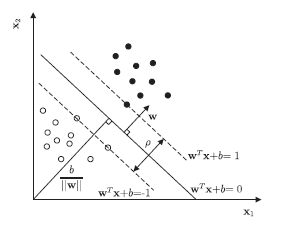
\includegraphics[scale=1.0]{gfx/SVM_1.PNG}
    \captionsetup{justification=centering}
	\caption{SVM hyperplane for binary classification of linearly separable data}
	\label{fig:SVM structure}
\end{figure}
Figure 1 \cite{DBLP:journals/tist/ChangL11} shows the basic principle of SVM for classification. Figure \ref{fig:SVM structure} depicts the bounding planes that are parallel to the hyperplane bordering each of the sub-classes and the data points that lie on the bounding planes called as support vectors \cite{DBLP:journals/tist/ChangL11}. For a given set of $n$ training samples ${x_i, y_i}$ such that $i \in n$ and each of the sample has $Q$ features ($x_i \in R^Q$) and class label with one of the binary values ($y_i \in \{-1, 1\}$), a hyperplane is a $n-1$ dimensional plane as:
\begin{equation}
    w^T x + b = 0
\end{equation}
where $w$ denotes a vector orthogonal to the hyperplane and $b$ is a constant\cite{DBLP:phd/dnb/Kimotho16}. Such a hyperplane
$(w, b)$ that separates data defines the function:
\begin{equation}
    f(x) = sgn(w^T x + b)
\end{equation}
In classifying problems, a larger margin $\rho$ means a better classification accuracy separating the two data classes and it involves minimizing $w$. A detailed derivation of binary classification of linearly separable data is described in paper by Kimotho\cite{DBLP:phd/dnb/Kimotho16}.

In the case of non-linearly separable data, SVM employs a kernel function as mentioned in table \ref{sec:SVM:Kernal} to transform the input data into a higher dimensional feature space where classification is carried out \cite{Burbidge2001AnIT}. 
\begin{table}[h]
    \centering
	\begin{tabularx}{\textwidth}{| X | X |}
		\hline
		\textbf{Kernal functions} & \textbf{$K(x_i,x_j)$}\\\hline
		Linear & $x_i^T x_j$\\ \hline
		Polynomial of power $p$ & $(1 + x_i^T x_j)^p$\\\hline
        Radial basis function & $exp(-\gamma || x_i - x_j ||^2)$\\\hline
        Multi-layer perceptron & $tanh(\gamma_0 x_i^T x_j + \gamma_1)$\\\hline
    \end{tabularx}
    \captionsetup{justification=centering}
	\caption{Kernal functions in SVM}
    \label{sec:SVM:Kernal}
\end{table}
\vspace*{-4mm}
The health state classification deals with the classification of more than one health states found during the degradation stages of machine lifetime, hence the multiple instances of binary SVM classifier is combined to achieve multi-classification. Strategies such as "One-Against-One(OAO)", "One-Against-All(OAA)" and "Directed Acyclic Graph SVMs" are used to perform the health state probability estimation of discrete failure degradation stages. A comparison of these strategies was done and OAO is found as leading over the other two in practical terms\cite{DBLP:journals/tnn/HsuL02}. In OAO, for given observations $x_t = (x_{t_1}, x_{t_2},...,x_{t_m})$, where $m$ is the number of observations in hand and $t$ is the timestep. Assuming $y_t$ as the health state at time $t$ and $y_t$ = 1,2,...,$n$, where n is the number of health states. For the multi-classification of $n$-health state events, the one-against-one method has $n(n-1)/2$ classifiers, where each classifier is trained on data from two classes. For training data from the $i^{th}$ and the $j^{th}$ classes, SVM solves the following classification problem:
\begin{equation}
\begin{split}
    minimize : 1/2 {|| w^{ij}||}^2 + C\sum_{t} \xi_j^{ij}(w^{ij})^T\\
    subject\:to: (w^{ij})^T \psi(x^t) + b^{ij}\geq 1 - \xi_j^{ij}, \; if y_t = i,\\
    (w^{ij})^T \psi(x^t) + b^{ij}\leq -1 + \xi_j^{ij}, \; if y_t = j,\\
    \xi_j^{ij} \geq 0 , \; j = 1, 2, ..., l
    \end{split}
\end{equation}

Here, the training data is mapped to a higher dimensional vector by function $\psi$ and $\psi(x^t)$ is considered as kernel function, $(x_t,y_t)$ is the $i^{th}$ or $j^{th}$ training sample, $w \in R^n$ is the coefficient vector, $b \in R$ is the bias
of the hyper-plane, $\xi_t^{ij}$ is the slack variable and $C$ is the penalty parameter. After a series of
tests, the decision is made using the following strategy: if sign $(w^{ij})^T \psi(x^t) + b^{ij}$ denotes $x_i$ to be in $i^{th}$ class then the class is added by one; otherwise, the $j^{th}$ value is increased by one.\newline
From the above SVM multi-classification result $(y_t)$, the probabilities of each health states $(S_t)$ is derived using the smooth window and indicator function $(I_i)$ as following: 
\begin{equation}
    \begin{split}
        Prob(S_t = i|\overrightarrow{x_t}, ..., \overrightarrow{x}_{t+u-1}) = \sum _{j=t}^{t+u-1} I_i(y_j)/u\\
        I_i = \left\{
        \begin{array}{ll}
          0, & \mbox{if $y \neq i$}.\\
          1, & \mbox{otherwise}.
        \end{array}
      \right.
    \end{split}
\end{equation}

As the probability of one state decreases, the probability of the next state increases. At the point of intersection there is a region of overlap between the two health states, which is a natural phenomenon in linear degradation process as depicted in Figure \ref{fig:SVM structure2}. However, the probability distribution of failure process is complex due to the dynamic and stochastic degradation process in a real world scenarios.
\begin{figure}[ht]
	\centering
	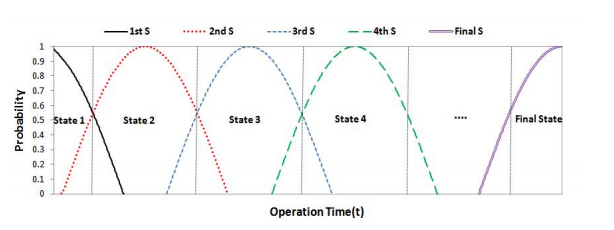
\includegraphics[scale=0.9]{gfx/svm_2.PNG}
    \captionsetup{justification=centering}
	\caption{Health state probability distribution for linear degradation process. \cite{Kim2010MachinePB}}
	\label{fig:SVM structure2}
\end{figure}

\subsection{Deep Belief Networks(DBN)}
\vspace*{-12mm}\hfill{\fontfamily{phv}\normalsize\emph{Anurose Prakash}}

Deep Belief Networks(DBN) classifier is one of the popular deep machine learning approaches that consists of a hierarchical structure with multiple layers of Restricted Boltzmann Machines (RBM). This approach utilises the advantages of deep learning such as fast inference and the ability to encode richer and higher order network structures \cite{DBLP:journals/ress/TamilselvanW13}. The author describes a DBN based health state estimation technique that has three consecutive stages:
\begin{enumerate}
    \item Collecting sensory data for DBN training and testing.\vspace*{-3mm}
    \item Developing DBN based classification models for the diagnosis of predefined health states.\vspace*{-3mm}
    \item Validating DBN classification models with testing sensory dataset\vspace*{-3mm}
\end{enumerate}
The structure of DBN is a layered architecture made up of multiple layers of RBMs with one visible layer and more than one hidden layer. 
\begin{figure}[ht]
	\centering
	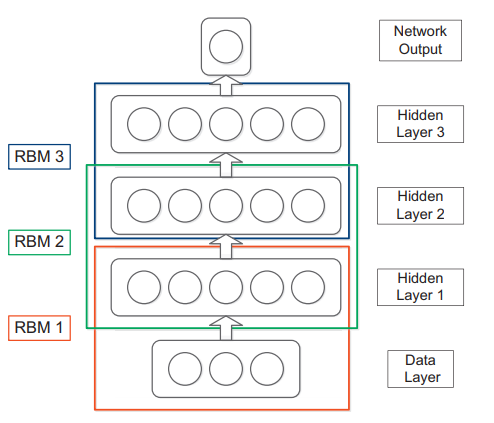
\includegraphics[scale=0.8]{gfx/dbn1.png}
    \captionsetup{justification=centering}
	\caption{DBN Structure.\cite{DBLP:journals/ress/TamilselvanW13}}
	\label{fig:DBN structure}
\end{figure}

\begin{figure}[ht]
	\centering
	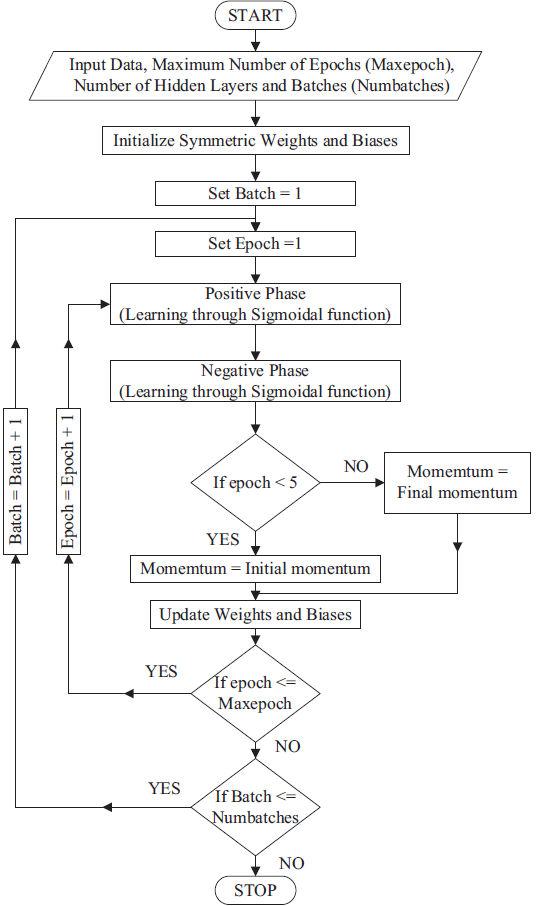
\includegraphics[scale=0.6]{gfx/dbn3.png}
    \captionsetup{justification=centering}
	\caption{Each iteration of RBM unit learning \cite{DBLP:journals/ress/TamilselvanW13}.}
	\label{fig:DBN_layer_structure}
\end{figure}
The visible layer of a DBN accepts the input data and transfers the data to the hidden layers. Figure \ref{fig:DBN structure} shows a DBN structure with 3 layers of RBMs. Layer 1 and layer 2 denotes the first RBM and similarly for the other layers. Each of the connected RBM layers undergoes the same transformation concept leading to a regular learning process within the structure. The training process of DBN involves two stages, i.e. training the RBM unit by means of the RBM learning rule and performing the back propagation supervised learning. The RBM learning rule consists of two steps - the positive and the negative phases as depicted in Figure \ref{fig:DBN_layer_structure}.
The positive learning phase transfers data from the bottom visible layer to the hidden layer and derives the probability of generating hidden units as $p(h|v,W)$. Its is formally defined as :
\begin{equation}
P(h_j = 1|v) = sigm ( -b_j - \sum_k v_k w_{jk} )    
\end{equation}

The negative phase operates as a reconstruction of the data from previous visible layer and determines the probability of generating visible units as $p(v|h,W)$ formally stated as:
\begin{equation}
P(v_k = 1|h) = sigm ( -b_k - \sum_j v_j w_{jk} )    
\end{equation}
\vspace*{-1mm}
Here, $w_{jk}$ denotes the synaptic weight updated as part of learning process in the respective positive and negative phases represented as:
\begin{equation}
    \Delta w_{jk} = \delta(\langle v_k h_j \rangle_{data} - \langle v_k h_j \rangle_{recon}) 
\end{equation}
where $\delta$ is learning rate and has values between 0 and 1, $\langle v_k h_j \rangle_{data}$ is pairwise product of the state vectors for the $j^{th}$ neuron in the hidden layer and the $k^{th}$ neuron in the visible layer after the positive phase learning process,whereas $\langle v_k h_j \rangle_{recon}$
denotes the pairwise product after the negative phase learning process for reconstruction of the visible layer. The overall system function of DBN learning procedure is defined as the probability of generating a visible vector ($v$) denoted as $p(v)$ which is function of weights and hidden vectors based on RBM learning rule as:
\begin{equation}
    p(v) = \sum_h p(h|v,W) p(v|h,W)
\end{equation}

The transformation function in the training process is sigmoid transformation that modifies the data from one layer to another and it is represented as:
\begin{equation}
    P(s_i = 1) = \frac{1}{1 + exp(-b_i - \sum_j s_j w_{ij})}
\end{equation}
where, $s_i$ and $b_i$ corresponds to the state and bias of $i^{th}$ neuron in the hidden layer, $s_j$ is the state of $j^{th}$ neuron in the visible layer and  $w_{ij}$ stands for synaptic weight between $i^{th}$ and $j^{th}$ neuron. Momentum $m$ is used for stabilizing the RBM learning process and it updates the synaptic weights and biases. The weight update of the current epoch gets updated with previous epoch as:
\begin{equation}
    \Delta w_{jk} = (m[\Delta w_{jk}]_{n-1}) + \delta(\langle v_k h_j \rangle_{data} - \langle v_k h_j \rangle_{recon})
\end{equation}
\begin{figure}[t]
	\centering
	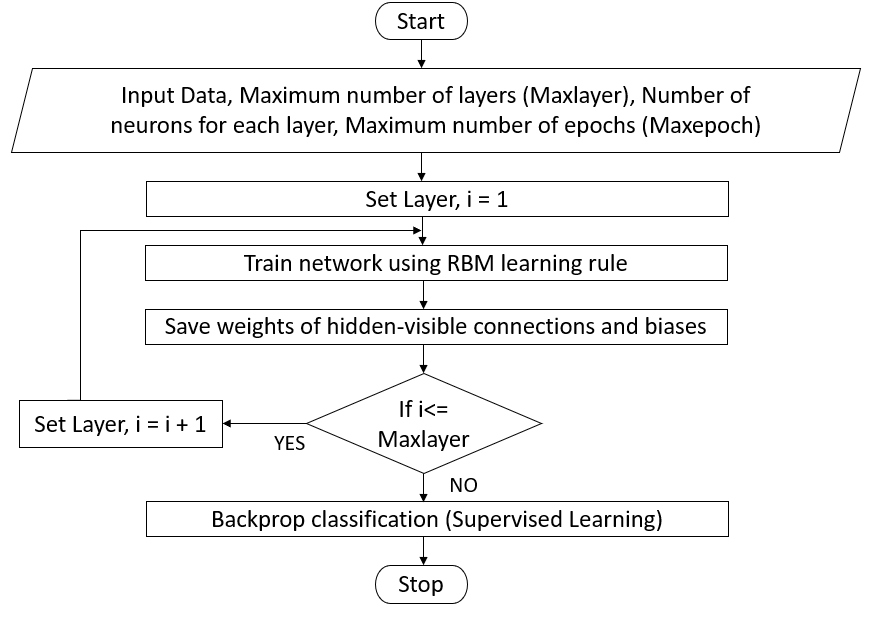
\includegraphics[scale=0.4]{gfx/Ed_dbn2.PNG}
    \captionsetup{justification=centering}
	\caption{DBN training process \cite{DBLP:journals/ress/TamilselvanW13}.}
	\label{fig:DBN_training_structure}
\end{figure}
As illustrated in Figure \ref{fig:DBN_training_structure}, the input to training model consisting of pre-processed batch data, the total number of layers in the DBN classifier model, the total number of hidden neurons in each hidden layer, and number of epochs are initialized. Within each layer of the training process, each of the involved RBM is individually trained and the weights and biases are saved for further analysis. Weights between visible and hidden layers and biases of the neurons in each DBN layer are optimized until the maximum number of epochs reached. The layer by layer training is followed by a supervised back-propagation training mechanism that considers all DBN layers simultaneously. The back-propagation learning is continued until the network output reaches the maximum number of epochs. This involves training the multi-layer neural network of the back-propagation network by computing error derivatives obtained after hidden layer activities and updating the weights as per requirement. Following this, the trained DBN classifier model can be further fine-tuned to improve the classification accuracy through certain fine-tuning algorithms. The weight file is used to determine the classification error.

\subsection{Logistic Regression (LR)}
\vspace*{-12mm}\hfill{\fontfamily{phv}\normalsize\emph{Anurose Prakash}}

Logistic Regression(LR) is a well-known classification model in ML with the lowest algorithm complexity. As this technique belongs to supervised learning, the collected data must have corresponding health state labels to be fed into the model. LR models have a close resemblance to the machine degradation process with its logic S-curve \cite{CAESARENDRA20101161}. This model is implemented with manifold regularization (LRMR), where it is further proposed for tool health assessment and online prediction\cite{DBLP:journals/asc/Yu18}. It is capable of estimating the failure time point of the tool with high accuracy and calculation efficiency. The logistic probability function for a logit model $g(x)$ is:
\begin{equation}
    P(x) = \frac{1}{1 + e^{-g(x)}}
\label{eq:lr}
\end{equation}
Given the n training samples, ${(x_i, y_i),
i = 1, ..., n}$, where each $x_i \in R^m$ is an m-dimensional feature vector,and $y_i \in \{0, 1\}$ is a class label, LR is defined as follows:
\begin{equation}
    log \frac{\pi_i}{1-\pi_i} = \beta_0 + \sum_{j=1}^m \beta_j x_{ij} \Leftrightarrow \pi_i = \frac{1}{1 + e^{-(\beta^T x_i)}}
\end{equation}
where $\pi_i$ denotes $p(y_i = 1|x_i,\beta)$, and $\beta$ = $(\beta_0, \beta_1, ...\beta_m)$ denotes the
vector of regression coefficients including a constant or intercept $\beta_0$. The prediction probability $P(x)$ of an event occurrence by LR is constrained between 0 and 1, which is considered as a health indication (HI) for quantifying the tool health state, i.e.,
\begin{equation}
HI_t = P(x_t)    
\end{equation}

where $P(x_t)$ can be calculated by using Eq. \ref{eq:lr}. The LRMR algorithm is used to construct LR to achieve the predicted LPs (i.e., $HI_t$). In order to improve the sensitivity and reliability of the HI (i.e., LP) to the slight degradation of tool health, the exponentially weighted moving average (EWMA) statistic of the LPs is used as an improved HI of tool health.

\subsection{Neuro-Fuzzy}
\vspace*{-15mm}
\hfill{\fontfamily{phv}\normalsize\emph{Saghar Heidari}}

The condition of a system or machine is in most cases not completely good or bad but something in between. Therefore, fuzzy logic helps to deliver this kind of uncertain knowledge in a way that is understandable for computers. Indeed, these kinds of approaches automatize the processes which should be done by a human in the past but still keeps the process interpretable and understandable using linguistic variables \cite{zeraoulia2005simple}.
The neural networks are good at reasoning tasks based on parallel computation and high speed and keep working in case of missing some piece of information while they are not able to explain how some certain decisions are attained. The fuzzy systems instead can explain system behaviors through rules and their performance can be modified by changing rules. As knowledge acquisition is in most cases not an easy task, the use of fuzzy systems is limited to the fields about which expert knowledge is available and the input data also is small.
The hybrid solutions like Neuro-Fuzzy Systems (NFS) combine both systems to get a more practical system. NFS is part of the soft computing concept.  
Neural networks can recognize patterns using a sufficient number of examples without prior knowledge. In contrary to neural networks, for fuzzy systems the prior knowledge, explicit linguistic rules, is needed if there is a lack of information or missing information the system should be tuned. In fact, neuro-fuzzy systems are neural networks that optimize certain parameters of fuzzy systems (e.g. membership function) or preprocess the data and extract fuzzy rules from data.\\
There are several types of NFS. The Mamdani-type and the Takagi-Sugeno-type \cite{Rutkowski2009} (also known as Adaptive Neuro-Fuzzy Inference System or ANFIS) neuro-fuzzy systems are the most famous types.

\subsubsection*{Fuzzy Systems:}
Every fuzzy system \cite{Rutkowski2009} consists of four components as follows (see Figure \ref{fig:Fuzzy Inference System}):\\\\
\textit{1: A fuzzifier}: It converts the input data into a fuzzy set.\\
\textit{2: A rule base}: It has fuzzy IF-THEN Rules which are provided by experts for making a decision.\\
\textit{3: A fuzzy inference engine}: It employs fuzzy reasoning techniques to determine the matching degree of input with respect to fuzzy IF-THEN rules.\\
\textit{4: A defuzzifier}: It converts the fuzzified output into crisp output.

\begin{figure}[H]
    \centering
    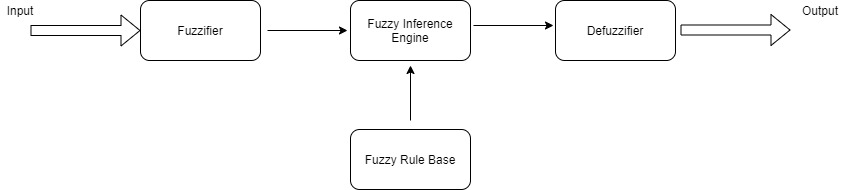
\includegraphics[width=14cm]{gfx/Fuzzy_Inference_System.png}
    %\vspace{0.3cm}
    \captionsetup{justification=centering}
    \caption{Fuzzy Inference System}
    \label{fig:Fuzzy Inference System}
\end{figure}

\subsubsection*{Formal Definitions:}
Given $x$ and $y$, as two linguistic variables (e.g. High Temperature and imminent Failure) are  $A$ and $B$, ${A}'$and ${B}'$ are fuzzified input and output accordingly the ${B}'$ can be resulted by fuzzified input ${A}'$ and relationship $R$, where relationship $R$ is \cite{Rutkowski2009}:
\begin{equation}
 IF\;\;\,  x\;\; is\,\, A\;\;\,  THEN\;\;  y\;\; is\,\, B   
\end{equation}

We face the challenge of estimating the membership function of the fuzzy relation denoted by:
\begin{equation}
    \mu _{{B}'}\left ( y \right )= \mu _{A\rightarrow B}\left ( x,y \right )
\end{equation}
Based on the knowledge of $\mu_{A}\left ( x \right )$ and  $\mu_{B}\left ( y \right )$ we can rewrite the membership function as follows:
\begin{equation}
    \mu _{A\rightarrow B}\left ( x,y \right )=I\left(\mu_{A}\left ( x \right ),\mu_{B}\left ( y \right ) \right)
\end{equation}

Figure \ref{fig:Different forms of membership functions} shows various type of membership functions.
\begin{figure}[H]
    \centering
    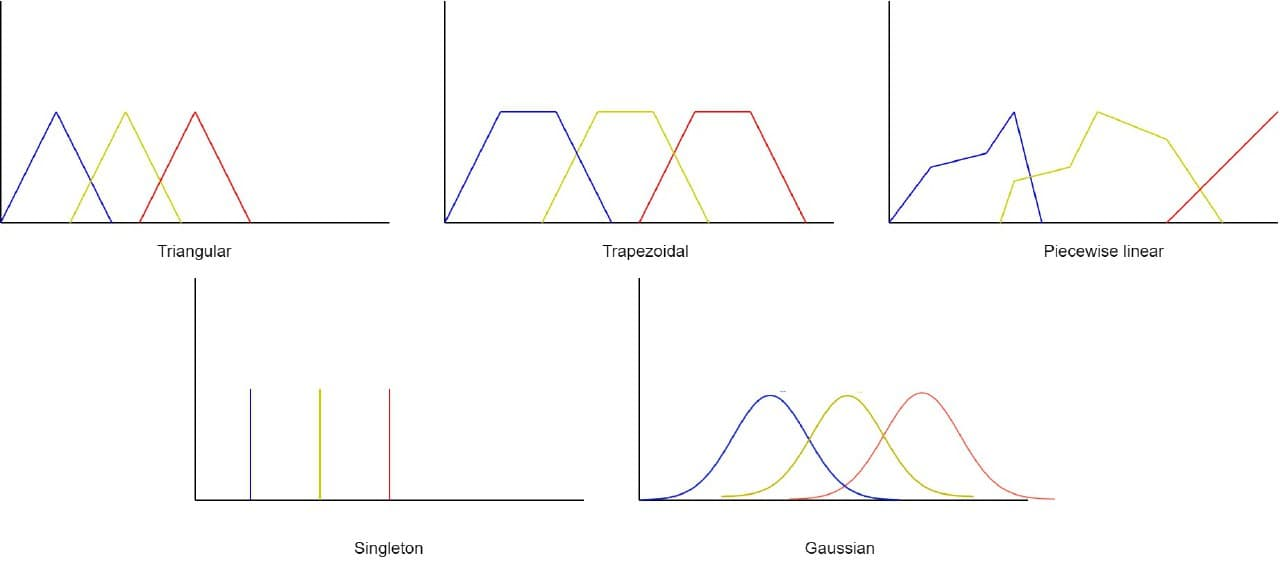
\includegraphics[width=12cm]{gfx/membership_function.png}
    \vspace{0.3cm}
    \captionsetup{justification=centering}
    \caption{Different forms of membership functions}
    \label{fig:Different forms of membership functions}
\end{figure}
\vspace*{-4mm}
We consider a multi-input-single-output fuzzy system. In health state classification normally we aim to classify a state based on the multi parameters to some specific state. The system maps $X\rightarrow Y$, where $X\subset R^{n}$ and $Y \subset R$ . As mentioned before, each fuzzy inference system consists of a fuzzifier, a fuzzy rule base, a fuzzy inference engine and a defuzzifier. Combining fuzzy inference system and neural network then we have a fuzzification layer, fuzzy rule base layer (in Mamdani Type, It called AND operation Layer), fuzzy inference layer and defuzzification layer. A fuzzifier maps $\bar{x}=\left[\bar{x_{1}},...,\bar{x_{n}}\right]\;\;\in X$ into a fuzzy set ${A}'\subseteq X$ characterized by a membership function $\mu_{{A}'}\left(x\right)$(e.g. a triangular or singleton membership function).
\\
The fuzzy rule base is a set of N fuzzy IF-THEN rules as follows:
\begin{equation}
   R^{\left ( k \right )} : \left\{\begin{matrix}
IF   & x_{1} \; is\; A_{1}^{k} & AND \\ 
     & x_{2}\; is\; A_{2}^{k} & AND \\ 
     & ...  & \\ 
     & x_{n}\; is\; A_{n}^{k} & \\
THEN & y\; is\; B^{k} & 
\end{matrix}\right. 
\end{equation} 
where
$$x=\left[x_{1},....,x_{n}\right] \in X,\,y\in Y,$$
$$A^{k}=A_{1}^{k}\times A_{2}^{k}\times ... \times A_{n}^{k}$$
are fuzzy sets characterized by membership functions $\mu_{A_{i}^{k}}\left(x_{i}\right),\;\;i=1,...,n,\;\;k=1,...,N$
and $B^{k}$ are fuzzy sets defined by membership functions $\mu_{B^{k}}\left (y\right),\;\;k=1,...,N$.
Then, the firing strength of the $k$th rule, $k=1,...,N$ is denoted as follows:
\begin{equation}
    \tau _{k}\left(\bar{x} \right )=\operatornamewithlimits{T}_{i=1}^{n}\left \{ \mu_{A_{i}^{k}}\left ( \bar{x}_{i} \right ) \right \}= \mu_{A^{k}}\left ( \bar{x} \right )
\end{equation}
Each of $N$ rules gives us a fuzzy set $\bar{B}^{k}\subseteq Y$ based on the compositional rule of inference.
\begin{equation}
    \bar{B}^{k}={A}'\circ \left(A^{K}\rightarrow B^{k}\right)
\end{equation}
Where $A^{k}=A_{1}^{k}\times A_{2}^{k}\times...\times A_{n}^{k}$ and fuzzy sets $\bar{B}^{k}$ are characterized by membership functions described by the sup-star composition:
\begin{equation}
   \mu_{\bar{B}^{k}}\left(y\right)=\operatornamewithlimits{sup}_{x \in X} \left \{ \mu_{{A}'}\left(x \right )\ast \mu_{A_{1}^{k}\times ... \times A_{n}^{k}\rightarrow B^{k}}\left(x,y \right ) \right \} 
\end{equation}
Where $\ast$ can be any operator in class t-norms (e.g. min operator $t\left( a,b\right)=min\left(a,b\right)$ or algebraic product $t\left(a,b\right)=ab$).\\
The aggregation operator for getting the fuzzy set ${B}'$ based on the fuzzy sets $\bar{B}^{k}$ is used which is the t-norm or t-conorm (e.g. $s\left(a,b\right)=max\left(a,b\right)$) depending on the type of fuzzy inference.
Finally, the defuzzifier maps from the fuzzy set ${B}'$ to a crisp point $\bar{y}$ in $Y\subset \mathbf{R}$ using COA (center of area) method as follows:
\begin{equation}
    \bar{y}= \frac{\int_{\mathbf{Y}}^{}y\cdot \mu_{{B}'}\left(y \right )dy}{\int_{\mathbf{Y}}^{}\mu_{{B}'}\left(y \right )dy}
\end{equation}
In the case of discrete systems, where $y^{-r}$ are centers of the membership functions $\mu_{B^{r}\left(y\right)}$ for $r=1,...,N$ the -crisp output $\bar{y}$ will be calculated as follows:
\begin{equation}
    \bar{y}=\frac{\sum_{r=}^{N}y^{-r}\cdot \mu_{{B}'}\left(y^{-r} \right )}{\sum_{r=1}^{N}\mu_{{B}'}\left(y^{-r} \right )}
\end{equation}
\begin{equation}
    \mu_{B}^{r}\left(y^{-r}\right)=\operatornamewithlimits{max}_{y\in\mathbf{Y}}\left\{\mu_{B^{r}}\left(y\right)\right\}
\end{equation}
\paragraph{Mamdani Neuro-Fuzzy Systems:}
In Mamdani-Type Neuro-fuzzy systems, the t-norm fuzzy implications are used (e.g. minimum or algebraic). The aggregation is performed by fuzzy union and in this case t-conorm. The fuzzy output set ${B}'\subseteq \mathbf{Y}$ using t-norm is calculated as follows:
\begin{equation}
    \mu_{{B}'}\left(y^{-r}\right)=\operatornamewithlimits{S}_{k=1}^{N}\left\{\mu_{\bar{B}^{k}}\left(y^{-r}\right)\right\}=\operatornamewithlimits{S}_{k=1}^{N}\left\{ T\left\{ \mu_{A^{k}}\left(\bar{x}\right),\mu_{B^{k}}\left(y^{-r}\right)\right\}\right\}
\end{equation}
The crisp output $\bar{y}$ is then:
\begin{equation}
    \bar{y}=\frac{\sum_{r=1}^{N}y^{-r}\cdot \operatornamewithlimits{S}_{k=1}^{N}\left \{ T\left \{ \operatornamewithlimits{T}_{i=1}^{n}\left \{ \mu_{A_{i}^{k}}\left ( \bar{x_{i}} \right ) \right \},\mu_{B^{k}}\left ( y^{-r} \right ) \right \} \right \}}{\sum_{r=1}^{N}\operatornamewithlimits{S}_{k=1}^{N}\left \{ T\left \{ \operatornamewithlimits{T}_{i=1}^{n}\left \{ \mu_{A_{i}^{k}}\left ( \bar{x_{i}} \right ) \right \},\mu_{B^{k}}\left ( y^{-r} \right ) \right \} \right \}}
\end{equation}
\paragraph{Takagi-Sugeno Neuro-Fuzzy Systems:}
This type of Neuro-fuzzy system is also known as adaptive neuro-fuzzy inference system (ANFIS) in which the rules have a fuzzy character in the IF part while the THEN part has functional dependencies. Therefore, the Rule base in ANFIS is as follows:
\begin{equation} 
\begin{split}
R^{\left(r\right)} & :\;IF \;\; \mathbf{x}\;is\;A^{r} \\
 & THEN\;\;y_{r}=f^{r}\left(x_{1},x_{2},...,x_{n}\right).
\end{split}
\end{equation}
At first we should implement fuzzy inference as follows:
\begin{equation}
    T\left(\mu_{A_{1}^{r}}\left(\bar{x_{1}}\right),\mu_{A_{2}^{r}}\left(\bar{x_{2}}\right),...,\mu_{A_{n}^{r}}\left(\bar{x_{n}}\right)\right),\;\;r=1,...,N.
\end{equation}
and then we have to compute:
\begin{equation}
    \bar{y_{r}}=f^{\left(r\right)}\left(\bar{x_{1}},\bar{x_{2}},...,\bar{x_{n}}\right),\;\;r=1,...,N
\end{equation}
and the output of ANFIS $\bar{y}$ is a normalized weighted sum of particular inputs $\bar{y_{1}},\bar{y_{2}},...,\bar{y_{N}}$:
\begin{equation}
    \bar{y}= \frac{\sum_{r=1}^{N}\bar{y_{r}}\operatornamewithlimits{T}_{i=1}^{n}\left \{ \mu_{A_{i}^{r}}\left ( \bar{x_{i}} \right ) \right \}}{\sum_{r=1}^{N}\operatornamewithlimits{T}_{i=1}^{n}\left \{ \mu_{A_{i}^{r}}\left ( \bar{x_{i}} \right ) \right \}}
\end{equation}
In the case of Takagi-Sugeno system with linear dependencies the rule base is as follows:
\begin{equation}
    \begin{split}
R^{\left(r\right)} & :\;IF \;\; \mathbf{x}\;\;is\;\;A^{r} \\
 & THEN\;\;y_{r}=c_{0}^{\left(r\right)}+c_{1}^{\left(r\right)}x_{1}+...+c_{n}^{\left(r\right)}x_{n}.
\end{split}
\end{equation}
\paragraph{Neuro-Fuzzy Systems considering Weights:}
we should distinguish between two kinds of weights regarding neuro-fuzzy systems:
(i)weights $w_{k}^{arg}\; \in \left[0,1\right], k=1,...,N$ describing the importance of each rule.\\
(ii)weights $w_{i,k}^{\tau}\in\left[0,1\right], k=1,...,N,i=1,...,n$ describing importance of antecedents or each linguistic variation of some input parameter $x_{i}$.  \\
Then we have two different rule base for each system as follows:
\begin{equation}
    R^{\left ( k \right )}:\begin{bmatrix}
IF & x_{1}\;\;is\;\;A_{1}^{k} & AND & ... \\ 
 AND& x_{n}\;\;is\;\;A_{n}^{k} &  & \\ 
 THEN& y\;\;is\;\;B^{k} &  & 
\end{bmatrix}\left ( w_{k}^{arg} \right ),
\end{equation}
\begin{equation}
    R^{\left ( k \right )}:\begin{bmatrix}
IF & x_{1}\;\;is\;\;A_{1}^{k}\left ( w_{1,k}^{\tau} \right ) & AND & ... \\ 
 AND& x_{n}\;\;is\;\;A_{n}^{k}\left ( w_{n,k}^{\tau} \right ) &  & \\ 
 THEN& y\;\;is\;\;B^{k} &  & 
\end{bmatrix}\left ( w_{k}^{arg} \right ).
\end{equation}\\\\
\textbf{Mamdani-Type and Takagi-Sugeno-Type Neuro-Fuzzy Systems Comparison:}\\
The main differences of Mamdani-Type and Takagi-Sugeno-Type neuro-fuzzy systems are as follows\cite{DBLP:journals/ijautcomp/EgajiGHY15}:\\
In Mamdani-type there is an output membership function and consequently, the output is a fuzzy set, while the output of Takagi-Sugeno-type is a constant or linear (weighted) expression. Sugeno-type is more complex in comparison to Mamdani-type, but Mamdani-type is more interpretable than the Sugeno-type.\\\\
Figure \ref{fig:Mamdani-Type Neuro-Fuzzy Architecture} shows the architecture of Mamdani-type neuro-fuzzy with 5 layers:\\\\
\textit{1.} Linear transformation layer\\
\textit{2.} Fuzzification layer\\
\textit{3.} AND-Layer where the rules are fired\\
\textit{4.} Fuzzy inference layer\\
\textit{5.} Defuzzification layer\\\\
In Takagi-Sugeno or ANFIS as shown in Figure \ref{fig:Takagi-Sugeno-Type Neuro-Fuzzy Architecture}, the two first layers are identical with the Mamdani-type neuro-fuzzy system but the third layer or rule layer is different. The IF-THEN rules in Mamdani-type are both fuzzy while in ANFIS just the IF part of rules are fuzzy and the THEN part is a function of input variables. The fourth layer of ANFIS is a normalization layer. Hence the implication method which is applied to Takag-Sugeno-type neuro-fuzzy system is the product t(a,b)=ab, the normalization layer is used to map the values of firing strength in [0,1] interval.\\ In the fifth layer, the output for each firing rule will be calculated and finally in the sixth layer, the sum of outputs of the fifth layer gives us the crisp final output of the neuro-fuzzy system.\\
\begin{figure}[H]
    \centering
    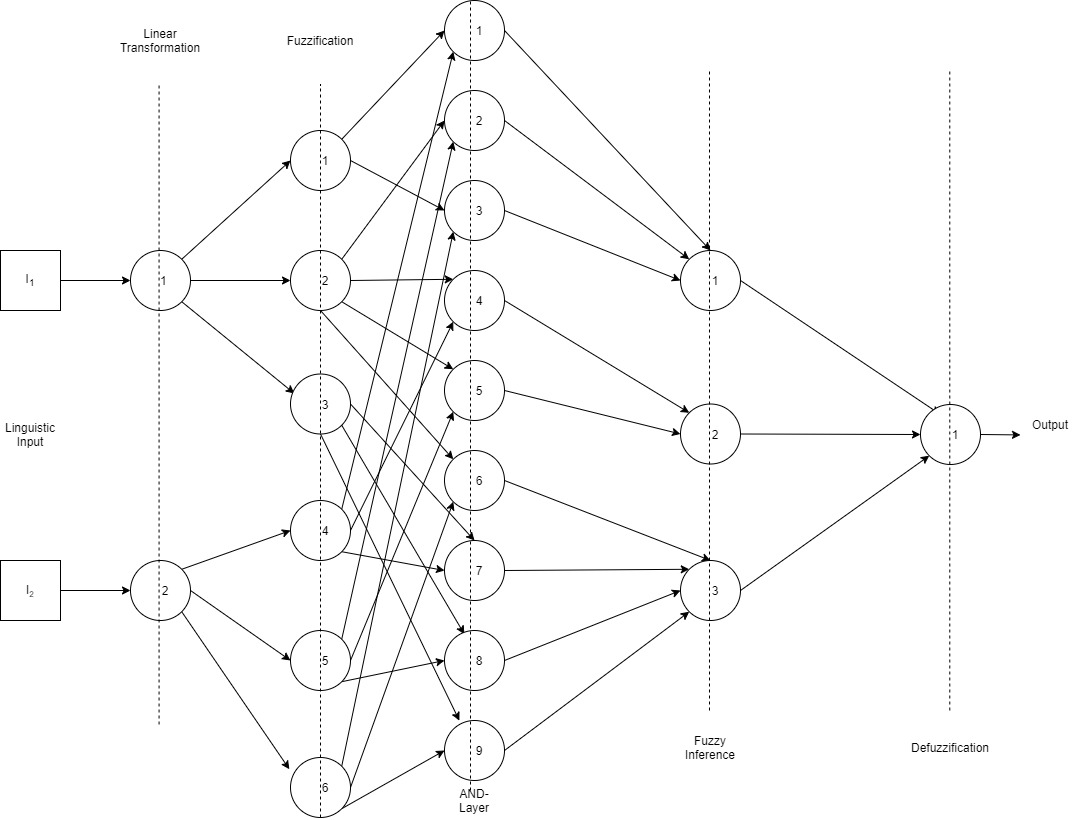
\includegraphics[width=14cm]{gfx/Untitled_Diagram.png}
    \captionsetup{justification=centering}
    \caption{Mamdani-Type Neuro-Fuzzy Architecture}
    \label{fig:Mamdani-Type Neuro-Fuzzy Architecture}
\end{figure}

\begin{figure}[H]
    \centering
    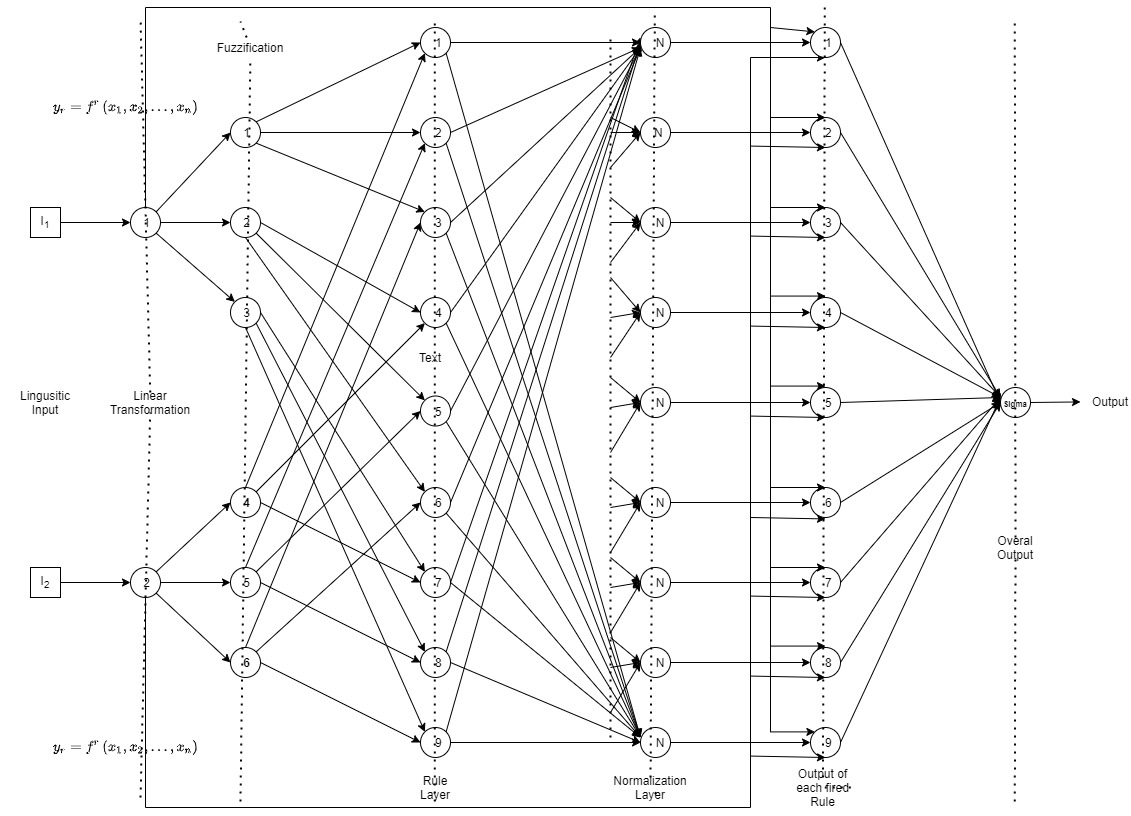
\includegraphics[width=14cm]{gfx/Takagi.png}
    \captionsetup{justification=centering}
    \caption{Takagi-Sugeno-Type Neuro-Fuzzy Architecture}
    \label{fig:Takagi-Sugeno-Type Neuro-Fuzzy Architecture}
\end{figure}


\subsection{Hidden Markov Models (HMMs)}
\vspace*{-15mm}
\hfill{\fontfamily{phv}\normalsize\emph{Saghar Heidari}}

Generally, predicting or estimating the health of a component in a mechanical system is one of the most challenges in condition based maintenance (CBM) for identifying and localizing machine failure (diagnostics). To address this problem, the Hidden Markov Model (HMM) is employed as a statistical markov model with unobserved (hidden) states for identification of the  current health state. Two kinds of regular HMM and hierarchical HMM are implemented as dynamic bayesian networks (DBNs) for health-state estimation \cite{DBLP:journals/tase/CamciC10, zhang2005integrated}.
 HMM has been used also in different fields, namely, automatic speech recognition (ASR), gen techniques, bioinformatics, handwriting recognition and partial discharges. Generally, the health-states are represented with probabilities because they can not be deterministic. The following equation shows the identified health state HS with the highest probability. Health -states affect observations, the sub-states and their transitions. Here, $X_{1:t}^{2}$ is sub-states from time 1 to $t$ and $X_{t}^{1}$ is health state at time $t$ \cite{DBLP:journals/tase/CamciC10}.
\begin{equation}
    HS=argmax_{S_{i}}(P(X_{t}^{1})=S_{i}|O_{1:t},X_{1:t}^{2})),\forall \;i,\;  i=1 ,\,2, \cdots ,N
\end{equation}
HMM uses time-series data that develop by a finite number of states which are hidden to outside observers and depend on the predecessor states. It is a process that produces a sequence of observable symbols as an output.
It consists of double stochastic processes:  A markov chain for the transition from one state to another in the hidden layer and the stochastic visible output in the observable layer. 

\subsubsection*{HMM Elements:}
HMM consists of several parameters \cite{camci2005dynamic, DBLP:journals/tase/CamciC10} that are listed as below :
\begin{enumerate}
    \item The state space S with N number of hidden states, $S=\left \{ S_{1},S_{2},\cdots,S_{N} \right \}$.\vspace*{-3mm}
    \item The set of observations is denoted as  
    $O=\left \{ O_{1},O_{2},\cdots,O_{T} \right \}$ which T is the number of observations in the sequence and $O_{t}$ denotes observations at time $t$. $O_{t}$ might be a discrete symbol  as $O_{t}\in \left \{ 1,\cdots ,L \right \} $ or a feature vector from L dimensional space , $O_{t}\in \mathbb{R}^{L} $.
    There exists also state sequence $X=\left \{ X_{1},X_{2},\cdots,X_{T} \right \}$  and $X_{t}$ is defined as health state at time $t$.\vspace*{-3mm}
    \item Transition matrix of state transition probability distribution expressed as $ A=\left \{  a_{ij}\right \}=P(X_{t}=S_{i}|X_{t-1}=S_{j})$ , $1\leq i,j\leq N$ which shows the probability of being in state $S_{i}$, at time t given that it is in state $S_{j}$ in time $t-1$.\vspace*{-3mm}
    \item Emission probability is called also observation probability distribution, $B=\left \{  b_{j}\left ( k \right )\right \}=P(O_{t}=k|X_{t}=S_{i}))$,  $1\leq i\leq N$ which defines the probability of observing k at time t given the state i.\vspace*{-3mm}
    \item The initial state distribution is the probability of being in state i when t=0 and is shown as $ \pi \left ( i \right )=P\left ( X_{1}=S_{i} \right )$ ,  $1\leq i\leq N$.
\end{enumerate}
    
The compact notation $\lambda =\left \{ A,B,\pi  \right \}$  for HMM is employed to show the complete parameter of model. Figure \ref{fig:HMM structure} shows the HMM structure.
\newline

\begin{figure}[H]
	\centering
	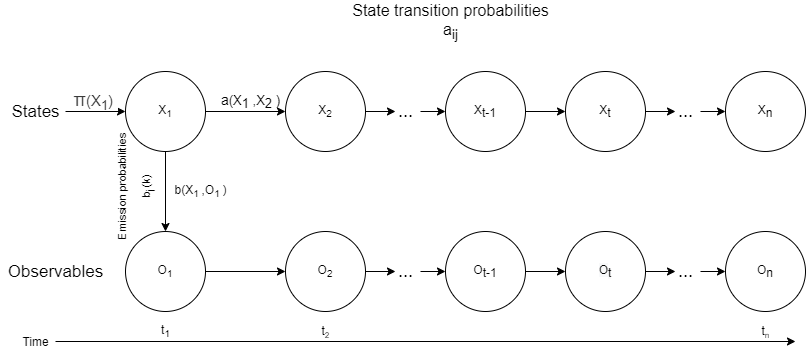
\includegraphics[width=12cm]{gfx/HMM.png}
    \captionsetup{justification=centering}
	\caption{Structure of Hidden Markov Model}
	\label{fig:HMM structure}
\end{figure}

\subsubsection*{HMM Problems:}
There are three main problems that can be solved by this model. These problems are the following:
\begin{enumerate}
\item{Evaluation Problem:}\\
The probability of the observation sequence  $O=\left \{ O_{1},O_{2},\cdots,O_{T} \right \}$ and  $\lambda =\left \{ A,B,\pi  \right \}$ is given.
The easiest way to calculate $P(O|\lambda )$ is the Brute-Force approach. Every state sequence of length $T$ is counted and the probability of each state sequence X given the model is calculated. First, hidden states denoted as $X=\left \{ X_{1},X_{2},\cdots,X_{T} \right \}$. Then, the emission probability B and transition matrix A, $\pi $ are used.
This approach solves the evaluation problem but it is too costly. The better way is the forward-backward (FB) algorithm \cite{DBLP:conf/interspeech/Bilmes98}, which is more efficient than direct evaluating. It uses forward variable $a_{t}(i)$ defined as
$a_{t}(i)= P( O_{1},O_{2},\cdots,O_{t} ,X_{t}=S_{i}|\lambda )$ which is the probability of partial observation sequence until time t and the state $S_{i}$ at step t given the model.\vspace*{-3mm} 
\item{Decoding Problem:}\\ The most likely state sequence that might produce the observation sequence is determined by using the Baum–Welch algorithm or the expectation maximization (EM) algorithm which utilizes both the forward and backward procedures \cite{DBLP:conf/icassp/Poritz88}.\vspace*{-3mm}
\item{Training Problem:}\\ The EM algorithm is used for solving the problem of adjusting the model parameters   $\lambda =\left \{ A,B,\pi  \right \}$   to maximize the likelihood of the observation sequence $P(O|\lambda )$).
\end{enumerate}

\subsubsection*{Implementation of HMM:}
The first step is to build an HMM for each state. For creating HMMs, it should be decided whether one HMM is used or a set of HMMs. Each state will represent a different health state when we have one HMM but in a set of HMMs, each HMM will be trained to express a different health state.
Then, a data sequence (observation sequence) is selected and the log-likelihood probability of obtaining this observation sequence given the HMM model is calculated for all HMMs $P(O|\lambda )$ through the FB algorithm. The HMM model with the highest log-likelihood value is selected as the best candidate for representing the health state and is allowed to further learn by using the current health state. Training continues until reaching the desired number of iterations for convergence. For testing, a test sequence as input is given to several trained HMM to compute the log-likelihood probabilities. The HMM model with the highest log-likelihood value is selected as the best candidate for representing the health state.
\paragraph{Dynamic Bayesian Network (DBN):}
It is an extension of bayesian network (BN) for modeling a system that is changing dynamically over time. DBN \cite{camci2005dynamic, DBLP:journals/tase/CamciC10} is designed to model probability distributions over sequence of random variables. It can handle sequenced observations that are generated by some hidden states evolving in time. DBN consists of two networks: a prior network which shows the prior probabilities of all variables in the network when $t = 0$ and a transition network which shows the probabilities of all the variables when $t = 1,2,...n$.
\paragraph{Dynamic Bayesian Network implementation of HMM:}
DBN shows the hidden-state as a set of random variables, while HMM has a single discrete random variable. DBN has two levels: observation level and hidden-state level \cite{camci2005dynamic}.
First, hidden-state $X_{t}$ and previous observation $O_{t-1}$ generate observation in time $t$ denoted as $O_{t}$. Then, a conditional probability distribution of each node given its parents is defined during the training process. These consist of initial probability distribution $P(X_{1}=i)$  , state transition distribution $P(X_{t}|X_{t-1})$, and the observation distribution $P(O_{t}|X_{t})$. Here, the observation distribution is considered as continuous and Gaussian:
\begin{equation}
P(O_{t}|X_{t}=i)\sim N(\mu_{i},\sigma _{i}^{2})
\end{equation}
As shown in Figure \ref{fig:DBN representation of HMM}, there are two different nodes in the hidden state level ($X_{1}$,$X_{t}$) in all-time slices $(t=1,2,...n)$ instead of M number of nodes. All the observations are represented by one node (O) since they have the same parent ($X_{t}$).
The purpose of a DBN performing as an HMM is to deduce the hidden-state given the observation sequence which is shown as $P(X_{t}=i|O_{1:t})$.
\begin{figure}[H]
	\centering
	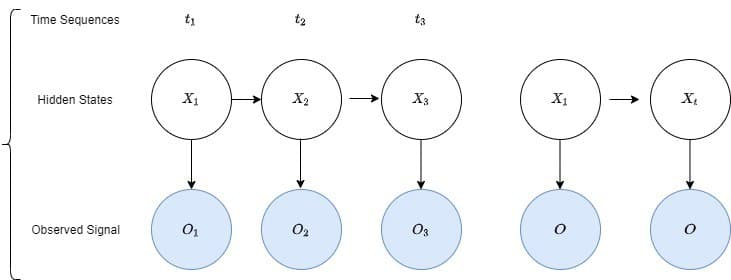
\includegraphics[width=10cm]{gfx/DBN_representation_of_HMM.png}
    \captionsetup{justification=centering}
	\caption{DBN representation of HMM}
	\label{fig:DBN representation of HMM}
\end{figure}

\subsubsection*{Hierarchical Hidden Markov Models:}
Hierarchical HMM (HHMM) is an extension of an HMM for modeling hierarchical structures for sequential data \cite{camci2005dynamic, DBLP:journals/tase/CamciC10}. Here, states include sub-states and both sub-states
and states. In an HHMM, the states also can produce single observations (production states) or strings of observations (abstract states). For instance, hidden states consist of the $t-th$ top-state denoted as  $X_{t}^{1}$ and  $X_{k}^{2}$ represents the $k-th$ sub-state. The transition between hidden states in the same level is horizontal transition. After sub-state transitions reach the last state, the health state transition occurs which is called vertical transition. Estimating the HHMM elements and model structure is more complex than HMM. DBN helps to represent HMMs in an efficient way by adding the flexibility of implementing different kinds of HMM like HHMM.

\paragraph{Dynamic Bayesian Network implementation of HHMM:}
In Figure \ref{fig:DBN representation of HHMM} , there is one arrow between the hidden-states in the top,  sub-state levels and the observation. There is also one arrow between top-level states and the sub-level state. When top-states for each sub-state is replicated, it makes a problem of losing the hierarchical structure. A binary control variable $F$ is used for solving this issue. If $F=1$, a top-level state changes and the lower-level state reaches its last possible state.
\begin{figure}[ht]
	\centering
	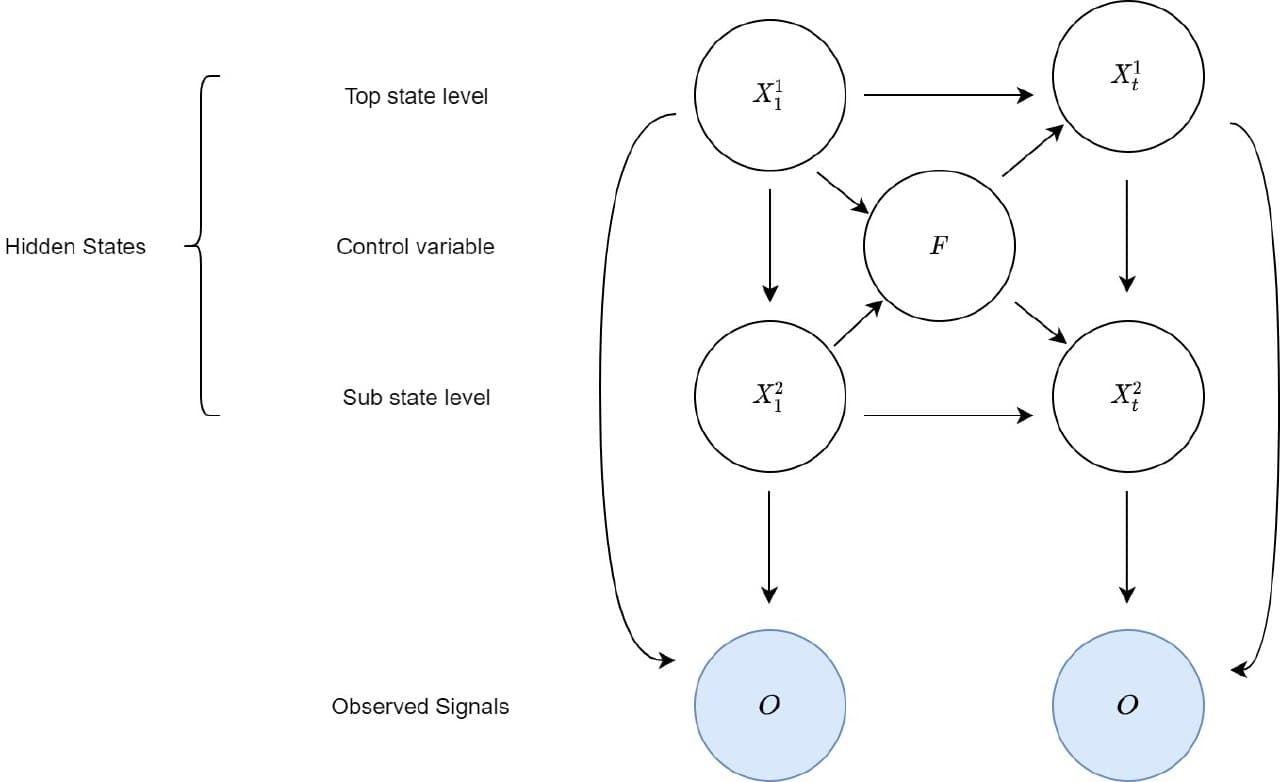
\includegraphics[width=10cm]{gfx/DBN_representation_of_HHMM.png}
    \captionsetup{justification=centering}
	\caption{DBN representation of HHMM}
	\label{fig:DBN representation of HHMM}
\end{figure}
The conditional probabilities of variables in the initial
time slice are initial distributions and are represented as:
\begin{equation}
    P(X_{1}^{1}=j)=\pi ^{1}(j)
\end{equation}
\begin{equation}
    P(X_{1}^{2}=i|X_{1}^{1}=j)=\pi_{j}^{2}(i)
\end{equation}
where $\pi ^{1}(j)$ is the initial top-level state distribution. When the upper state is in state $j$, the probability of sub-state being in state i denoted as $\pi_{j}^{2}(i)$. In this work, we have a vertical transition if $F=1$, otherwise we have a horizontal transition.
 The conditional probability distribution is shown in the next equation. Here, $A^{1}(i,j)$ is the top-level state transition probability from top state $i$ to $j$ if $F=1$.
\begin{equation}
P(X_{t}^{1}=j|X_{t-1}^{1}=i,F_{t-1}=f)=\begin{cases}
1 ,& \text{ if } f=0 , i=j \\ 
0, & \text{ if } f=0 , i\neq j \\ 
A^{1}(i,j),& \text{ if } f= 1
\end{cases}
\end{equation}
 In the sub-state level, the conditional probability in the sub-state level is based on either the initial distribution or the transition distribution depending on $F$.
\begin{equation}
 P(X_{t}^{2}=j|X_{t-1}^{2}=i,F_{t-1}=f,X_{t}^{1}=k)=\begin{cases} 
A_{k}^{2}(i,j),& \text{ if } f= 0 \\ 
\pi_{k}^{2}(j) ,& \text{ if } f=1 \\ 
\end{cases}
\end{equation}
If the high-level state is in $k$, the transition probability from state $i$ to $j$ is $A_{k}^{2}(i,j)$ and the initial sub-state level distribution is $\pi_{k}^{2}(j)$. The probability
of turning $F$ “on” ($F=1$) is equal to the probability of transition to the last state $l$.
\begin{equation}
    P(F_{t}=1|X_{t}^{1}=k,X_{t}^{2}=i)= A_{k}^{2}(i,l)
\end{equation}
The conditional distribution of the observed state is shown in next equation,
\begin{equation}
P(O_{t}|X_{t}^{1}=i,X_{t}^{2}=j)\sim N(\mu _{i,j},\sigma _{i,j}^{2})
\end{equation}



\subsection{K-Nearest Neighbors model (KNN)}
\vspace*{-12mm}
\hfill{\fontfamily{phv}\normalsize\emph{Saghar Heidari}}

K-Nearest Neighbors model is a non-parametric machine learning model that is used for classification and regression problems. This multi-class algorithm is also used for identifying the health condition of a system \cite{hasan2020health}. KNN works based on a similarity measure (minimum distance) and has two phases: 
In the training phase, the nearest neighbors are determined(see below in the KNN algorithm ). In the testing phase, predicted classes are compared to given class labels of test data. The goal of this approach is to predict the class for new input data based on the classes of available training data.
The KNN Algorithm employs distance measures like the standard Euclidean distance, Manhattan, and Minkowski distance. These metrics are used to find the nearest neighbors of an observation which is classified by its K nearest neighbors and the distances. The equation for calculating distance of two points
($X=\left \{ x_{1},x_{2},...,x_{n} \right \}$, $Y=\left \{ y_{1},y_{2},...,y_{n} \right \}$) with n elements is shown as below:
\begin{itemize}
\item  Euclidean distance : 
\begin{equation}
D(X,Y)=\sqrt{\sum_{i=1}^{n}}(x_{i}-y_{i})^{2} 
\end{equation}
\vspace*{-4mm}
\item  Manhattan distance: 
\begin{equation}
    D(X,Y)=\sum_{i=1}^{n}\left | x_{i}-y_{i} \right |
\end{equation}
\vspace*{-4mm}
\item Minkowski distance:
\begin{equation}
D(X,Y)=\left (\sum_{i=1}^{n}\left | x_{i}-y_{i} \right | ^{q} \right )^{1/q}
\end{equation}
\vspace*{-4mm}
\end{itemize}
\subsubsection*{KNN algorithm:}
The algorithm of KNN works as follows:
\begin{enumerate}
    \item Select the value k which determines how many nearest neighbors should be considered.
    \vspace*{-3mm}
    \item Calculate the distance between new input data and training samples via a distance function as defined above.
    \vspace*{-3mm}
    \item Sorting out the calculated distance in ascending order.
    \vspace*{-3mm}
    \item Choose k nearest neighbor from the sorted list.
    \vspace*{-3mm}
    \item Assign a class to the new data point which is a majority among its neighbors.
    \vspace*{-3mm}
\end{enumerate}
Figure \ref{fig:Example of KNN algorithm} shows the example of the KNN algorithm, in which the new sample is classified based on its neighbors. 


\begin{figure}[H]
	\centering
	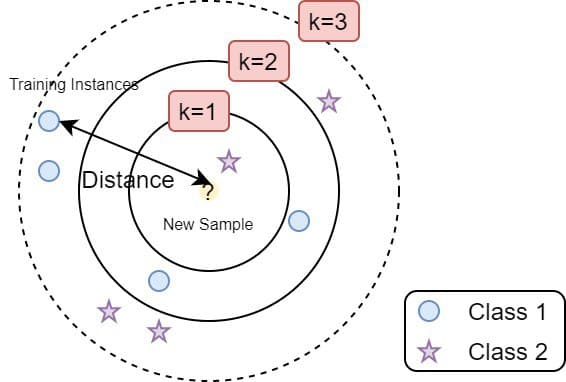
\includegraphics[width=8cm]{gfx/KNN.png}
    \captionsetup{justification=centering}
	\caption{Example of KNN algorithm}
	\label{fig:Example of KNN algorithm}
\end{figure}



\section{Evaluation setup}

\label{sec:system:sec5}

There are two main aspects that should be considered in the evaluation of a model. First, the model parameters by which the model performs at its best, which is also known as Hyperparameter tuning. Second, the performance of the model or how good is the model in predicting the target values (e.g. accuracy of the model).

\subsection{Score based evaluation metrics}
\vspace*{-12mm}
\hfill{\fontfamily{phv}\normalsize\emph{Saghar Heidari}}

To evaluate a classification model, there are some aspects that should be considered. First, The number of classes in the model. If we have to deal with a binary classification model or a multi-class classification model. Second, the distribution and importance of classes, which means if the data points for different classes are almost the same or most of the data points are classified for some specific class (balanced or imbalanced datasets). Whether the classes are equally important or some specific class is more important than the others. Based on such considerations, while an evaluation metric can describe some specific model precisely at the same time the same metric can be misleading for another model. In the following, we describe the well-known and well-established evaluation metrics and the usefulness of each for different classification tasks \cite{DBLP:journals/prl/FerriHM09, hasan2020health}.

\paragraph{Confusion Matrix:}
It is a Matrix that compares actual values of the target parameter and the predicted values for instance in the case of binary classification the confusion matrix consists of 4 categories as follows \cite{DBLP:journals/corr/BrancoTR15, article}:
\begin{enumerate}
\item{True Positive (TP):} the class is predicted as a class (+) and the actual class is (+). \vspace*{-6.5mm}
\item{False Positive (FP):} the class is predicted as a class (+) but the True class is (-). \vspace*{-6.5mm}
\item{True Negative (TN):} the class is predicted as a class (-) and the actual class is (-). \vspace*{-6.5mm}
\item{False Negative (FN):} the class is predicted as a class (-) but the actual class is (+).
\end{enumerate}

\paragraph{Normalized Confusion Matrix:}
Calculates the percentage of each category regarding a total number of predictions e.g. if the number of prediction is N=(TP+FN+FP+TN) then:
\begin{enumerate}
    \item $0\leq \frac{TP}{N} \leq 1$ \vspace*{-3mm}
    \item $0\leq \frac{FP}{N} \leq 1$ \vspace*{-3mm}
    \item $0\leq \frac{TN}{N} \leq 1$ \vspace*{-3mm}
    \item $0\leq \frac{FP}{N} \leq 1$ \vspace*{-3mm}
\end{enumerate}
\paragraph{Accuracy:}
It is defined as the number of correctly predicted values divided by the total number of all values. Using confusion matrix in binary classification we can define accuracy as follows:
\begin{equation}
    Accuracy= \frac{TP+TN}{TP+TN+FP+FN} 
\end{equation}

\paragraph{Precision:}
The percentage of correctly predicted positive class out of all positive predicted values.
\begin{equation}
Precision = \frac{TP}{TP+FP}    
\end{equation}

\paragraph{Recall:}
Recall also known as sensitivity in medical science and true positive rate.
The number of correctly predicted positive class (+) divided by the number of values in the positive class.
\begin{equation}
   Recall\;(TP_{rate}) = \frac{TP}{TP+FN}
\end{equation}
\paragraph{Specificity:}
It is the number of correct predictions of the negative class (-) or TN divided by the actual number of values in the negative class.
\begin{equation}
    Specificity\;(TN_{rate})=\frac{TN}{TN+FP}
\end{equation}
The following equation shows the calculation of False Positive Rate (FPR).
\begin{equation}
    FP_{rate}=\frac{FP}{TN+FP} 
\end{equation}

\paragraph{F1-Score:}
This score considers both precision and recall simultaneously and hence computes the harmonic mean of precision and recall as follows:
\begin{equation}
    F1-Score = 2\times \frac{Recall\times  Precision}{Recall+  Precision}
\end{equation}
\paragraph{ROC and AUC:}
The Receiver Operator Characteristic (ROC) and the Area Under The Curve (AUC) curve are evaluation metrics for checking the performance of classification problems.
ROC is plotted by TPR against FPR (on axis y and x respectively). The more the curve shifted toward the left top corner, the better the model can distinguish between two groups and the more the curve shifted toward indifferent or arbitrary line (the diagonal where x=y), the weaker is model in differentiating between two groups. The greater is the AUC or the area under the ROC curve, the model is better.

\paragraph{Metrics for multiclass classification:}
In this case for the calculation of metrics like precision and recall and F1-Score, we should use the principle of one-against-others which means each time we consider a class as a positive class and the other classes as a negative class and repeat it for all classes. Then, the calculation of metrics would be as same as for binary classification.
There are 3 more metrics for multiclass classification problem as follows \cite{grandini2020metrics}:
\begin{enumerate}
\item Micro-F1: Micro average considers total values of TP, FP, FN regardless of which class they belong to and then computes precision, recall as well as F1-Score as expected the values of precision and recall and Micro-F1 are same.
\item Macro-F1: It computes F1-scores of each class and then take unweighted average of them (without consideration of the number of each class). 
\item Weighted-F1: It takes the frequency of each class into account.
Applying the same principle (binarization of a multiclass classification), the Roc curves for a multi class classification can be obtained.
\end{enumerate}
\paragraph{Balanced and imbalanced data:}
In health state classification, we normally deal with imbalanced datasets. In most cases, the majority of data points represent the normal or healthy class and the classes have different levels of importance. Classes that represent sudden failure are more important than classes that represent gradual failures.
One common approach for binary classification is to tag minority class as positive class and then calculate some metrics as sensitivity or specificity \cite{DBLP:journals/corr/BrancoTR15, article}.

\textit{1. F-Beta-Score:} F1-score is one of the popular metrics for imbalanced classes but as the importance of false Positive and false negatives can be different, the F-Beta-Score is introduced, in which different weights will be assigned for false positives and false negatives. For instance, F-0.5-Score and F-2-Score give more weights for positive class and negative class respectively.
\begin{equation}
 F_{\beta } =\frac{(1+\beta ^{2})\cdot (precision\cdot recall )}{(\beta ^{2}\cdot precision+ recall)}
\end{equation}
\textit{2. Precision-Recall Curve:} This is another metric that is quite similar to the ROC curve but is useful in the case of imbalanced data. Precision-Recall curves have the recall and precision rates expressed on the axes. The precision on the y-axis plotted against Recall on the x-axis. The better classifiers tend to right top corner and the arbitrary classifiers is a horizontal line (y=0.5). The area under Precision-Recall curve as AUROC curve (Area Under the Receiver Operating Characteristics) can be used for comparison of different classifiers.



\subsubsection{Calibration scores}
\vspace*{-12mm}\hfill{\fontfamily{phv}\normalsize\emph{Anurose Prakash }}

In most of the cases of supervised health state estimation, the health state is assigned based on the probabilistic models. These models yield a probability membership of a data sample to each of the possible class groups in the problem, $\widehat{p}(c|x)$. By setting a discriminatory threshold, it is possible to select one of the class assignments. However, the evaluation of the classification process by means of standard scores (Accuracy, Recall, etc.) disregards the information about the uncertainty in-class assignment. By contrast, calibration scores aim to measure how close the probability assignment given by the classifier is from the true distribution of the class. Thus, calibration scores incorporate classifier uncertainty in the assessment of the classification performance. Among the best-known calibration scores for classification is the Brier score, which is defined as:

\begin{equation}
BS = \frac{1}{N} \sum_{i=1}^N \sum_{j= \{c^+, c^-\}}(\widehat{p}(C = j|x^{(i)} - \delta(j,c^{(i)}))^2  
\end{equation}
where $\widehat{p}(C = j|x^{(i)})$ is the probability assigned by the classifier to the $i^{th}$ instance for class group $j$ and $\delta(j, c(i))$ is a Kronecker delta which equals 1 if the class
label for the $i^{th}$ instance is $j$ and 0 otherwise. Therefore, the Brier score is useful in problems where the interest lies in fitting the data distribution or in problems where experts perform class assignments on the basis of the expected probability class membership. Similarly, another well-known score used in calibration is the log loss:
\begin{equation}
Log Loss = \frac{1}{N} \sum_{i=1}^N \sum_{j= \{c^+, c^-\}} \delta(j,c^{(i)}) \log_2(\widehat{p}(C = j|x^{(i)}))
\end{equation}


\subsection{Generalization from binary to multi-class classification problems}
\vspace*{-12mm}
\hfill{\fontfamily{phv}\normalsize\emph{Anurose Prakash}}\newline

Evaluation metrics such as accuracy, classification error, Brier score and log loss can be straightforwardly extended to problems with multiple class labels. But, this is not the case with other scores
(e.g. recall, precision, etc.) and graphical methods (e.g. ROC curves, lift graphs,
etc.) as they can not be used directly in multi-class problems because they are based on
the presence of only two classes: positive and negative \cite{article}. Hence, the generalization schemes are used to reduce multi-class problems to a set of binary classification problems in order to use the presented scores in multi-class problems. Such
generalization schemes are OVA (one vs. all) and OVO (one vs. one).
\paragraph{OVA:}
Given that the class variable can take $r_C$ values, for each one of these binary problems is assigned a class value ($c_i$ with $i$ = 1,...,$r_C$) as the positive class and the rest of the class values are considered to belong to the negative class. Hence, $r_C$ scores (one for each binary classification problem) are produced denoted as $S_i$ with $i$ = 1,...,$r_C$ and the OVA score is obtained as follows:
\begin{equation}
    S_{OVA} = \sum_{i=1}^{r_C} p(c_i) . S_i
\end{equation}
\paragraph{OVO:}
Given that the class variable can take $2^{r_C}$ values, for each problem only those samples assigned to $c_i$ and $c_j$ class labels are considered with $i, j$ = 1,...,$r_C$ and $i < j$). Thus, $c_i$ is taken as the positive class and $c_j$ as the negative class to calculate the score, $S_{i,j}$ . Finally, the score is calculated as follows:
\begin{equation}
    S_{OVO} = \frac{1}{2^{r_C}}\sum_{i=1}^{r_C-1}\sum_{j=i+1}^{r_C} S_{i,j}
\end{equation}
%\begin{figure}[htb]
%	\includegraphics[width=\textwidth]{gfx/Clean-Thesis-Figure}
%	\caption{Figure example: \textit{(a)} example part one, \textit{(c)} example part two; \textit{(c)} example part three}
%	\label{fig:system:example1}
%\end{figure}

%\Blindtext[1][2]

% \section{System Section 2}
% \label{sec:system:sec2}

% \Blindtext[1][2]

% \begin{figure}[htb]
% 	\includegraphics[width=\textwidth]{gfx/Clean-Thesis-Figure}
% 	\caption{Another Figure example: \textit{(a)} example part one, \textit{(c)} example part two; \textit{(c)} example part three}
% 	\label{fig:system:example2}
% \end{figure}

% \Blindtext[2][2]

% \section{System Section 3}
% \label{sec:system:sec3}

% \Blindtext[4][2]

% \section{Conclusion}
% \label{sec:system:conclusion}

% \Blindtext[2][1]
